

\documentclass[conference]{IEEEtran}

\usepackage[nolist]{acronym}
\usepackage[backend=bibtex]{biblatex}
\usepackage{graphicx}
\addbibresource{sdn.bib}
% correct bad hyphenation here
\hyphenation{op-tical net-works semi-conduc-tor}


\begin{document}
	%
	% paper title
	% can use linebreaks \\ within to get better formatting as desired
	\title{Comparing caching approaches with \ac{sdn} for \ac{iot} applications}


	% author names and affiliations
	% use a multiple column layout for up to three different
	% affiliations
	\author{\IEEEauthorblockN{Florian Weidner}
		\IEEEauthorblockA{Philipps-University Marburg, Germany\\
			Department of Mathematics and Computer Science, Distributed Systems Group\\
			February 09, 2024\\
	}}

	% make the title area
	\maketitle

	\begin{abstract}
	%\boldmath
	The abstract goes here.
	\end{abstract}

	\begin{IEEEkeywords}
	\ac{sdn}, \ac{iot}, caching
	\end{IEEEkeywords}

	\IEEEpeerreviewmaketitle

	\section{Introduction}
	\label{section:introduction}

	With the development of the internet and the increasing complexity of networks, the management and configuration of them become more complex and time consuming. Technologies like moblie networks, cloud computing, multimedia applications and virtualization have a high need of bandwidth, high accessibility and dynamic network configurations. These requirements are a challenge for traditional networks. 

	Traditional Networks are very hardware-centric. Routers and switches are used to manage the network traffic. The control plane is very tightly coupled with the forwarding by the data plane. Since both are happening on the local device, the configuration and management of the network is very time consuming. \acf{sdn} addresses these issues. It uses a centralized approach for managing the network devices. This leads to easier configuration, more flexible forwarding, enhanced performance and reduced costs. \cite{Jefia2018-pj} \cite{MASOUDI20161}


	In this paper we will first summerize the concept of \ac{sdn} and look at applications and challanges In Section \ref{section:sdn-iot} we will focus on the usage of \ac{sdn} in \ac{iot} applications. In Section \ref{section:caching} we then deep dive even more into caching approaches with \ac{sdn} for \ac{iot} applications. Multible caching strategies will be compared. Finally, we will conclude our findings in Section \ref{section:conclusion}. 

	\section{\ac{sdn}}
	\label{section:sdn}

	\begin{figure}
		\label{fig:architecture-compare}
		\centering
		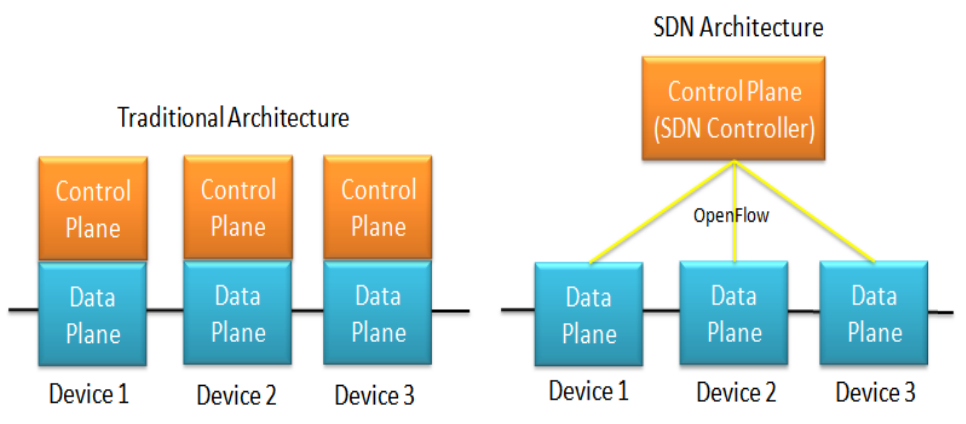
\includegraphics[width=0.5\textwidth]{figures/architecture-compare.png}
		\caption{Traditional Architecture and \ac{sdn} Architecture \cite{Jefia2018-pj}}
	\end{figure}

	\begin{figure}
		\label{fig:flow-table}
		\centering
		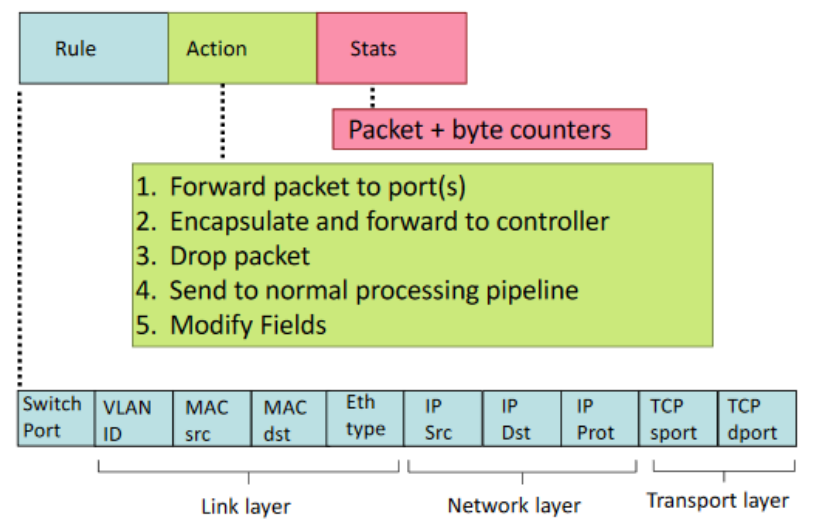
\includegraphics[width=0.5\textwidth]{figures/flow-table.png}
		\caption{Flow Table Entry Representation \cite{nunez2023briefoverviewsoftwaredefinednetworking}}
	\end{figure}

	\begin{quote}
		"\acf{sdn} is an emerging network architecture
		where network control is decoupled from forwarding and is directly programmable" \cite{sdn-onf} 
	\end{quote}

	This definition is by the \ac{onf} from 2012. \acf{sdn} decouples the control form the data plane. It uses a centralized controller, which has a global view to the network to manage the control plane. The controller can manage and adjust the network and the forwarding configuration of the network devices. There exist different implementations of \ac{sdn} controllers. In \ref{fig:architecture-compare} you can see the difference in the architectures of traditional networks and \ac{sdn} networks. In the traditional architecture, each device has its own control plane to manage the device. In \ac{sdn} the control plane is centralized using the \ac{sdn} controller.

	The main responsitblity of the data plane is forwarding the network traffic. For that, it uses flow tables to determin the forwarding desitnation, which are more complex forwarding tables of traditional routers or switches. More complex decisions based on the information of incoming packtes are possible. In \ref{fig:flow-table} you can se the representation of a flow table entry. An Entry contians three columns. The first one contains the rules to match the incoming packages. The rules can be applied to any part of the datagram. The second one are the actions, that should be executed if the rule matches. The third column is used to store performance metrics on their corresponding rule and action field. \cite{nunez2023briefoverviewsoftwaredefinednetworking}
	The dataplane can also be used, to enable various functions like network inspection, anomaly detection or traffic engineering. \cite{MASOUDI20161} 
	The third plane is the application plane. On that plane software is used to manage the network over the \ac{sdn} controller. There complex funtions can be performed to configure or automate the network trafic, based on the customer needs. \acp{api} are used to comunicate with the hardware in the network.

	The three planes use dedicated interfaces to comunicate. The southbound interface is used to comunicate between the control plane and the data plane. The northbound interface is used to comunicate between the control plane and the application plane. The OpenFlow Protocol, maintained by the \ac{onf} is a commonly used open-source protocol defining an interface for the southbound communication between the controller and the network devices. It defines guidelines and uses \ac{tcp} to update the flow table entires from the control plane. 
	If the controller is distributed the east-westbound \acp{api} can be used to comunicate between the controllers. \cite{nunez2023briefoverviewsoftwaredefinednetworking}


	\subsection{Advantages and Challenges of \ac{sdn}}

	\acf{sdn} has compared to traditional networking several advantages. Here the some of them are summerized.\ac{sdn} provides a better and easier management of the network. All network devices can be controlled from a single point. Also newlly added devices can be easily integrated into the network. \cite{Jefia2018-pj}
	Also the performance of the network will be imporved. It is possible to orchistrate the network traffic centrally. This leads to a better dynamic utilization of the network resources. This also leads to reduced costs. The management of the network is more efficient by using a central software, since there is less need to acces the individual network devices directly. \cite{Jefia2018-pj}
	The forwarding network devices can be simplified. They only need to be able to forward the network traffic and have basic functions to be able to execute the instructions of the contorller, which takes over the management logic. \cite{Hussain2022-tc} With \ac{sdn} the network gets programmable with applicaitons that are installed ot the control plane. The control plane can be dircetly programmed, since it is seperated from the data plane. That also makes automation possible. \cite{Hussain2022-tc}

	But \ac{sdn} also faces some challenges. Research into \ac{sdn} mainly focused on the control plane. The programability of the dataplane is not as advanced as the control plane. With OpenFlow, there is no solution provided for data plane customization. \cite{MASOUDI20161}
	For forwarding devices have a tradoff in flexibilty and performance. General purpose processors provide the highest flexibilty wheras specific standard products are specialized for high performance but lower flexibilty. \cite{Jefia2018-pj}New \ac{sdn} switches are using hardware combinations to achive a better balance between flexibilty and performance.  \cite{MASOUDI20161}
	\ac{sdn} networks are dependent on OpenFlow compatible switches, which limits the scalability. Also the controller needs to be distributed to achive further scalabiltiy, over the limits of a single controller. Splitting the controller leads to typical distributed system problems like latency, fault tolerance, consistency and load balancing. On the other and it also leads to more resilicance, performance and availability. \cite{MASOUDI20161} 
	Since \ac{sdn} is widely being adopted and used, security is getting very important. Controllers are a central target for security threads. With unauthorized access to the controller, the whole network can be compromised. Authentication between controllers and their network devices with \ac{tls} lighten these threads. To achive a secure network protection, an effective security model is mandatory. \cite{Jefia2018-pj}


	\subsection{Applications of SDN}

	SDN networks are used for data centers, enterprise networks, optical networks and even home and small buisinesses. \ac{sdn} enables customization and deployment of new services or policies, because the independence of the control and the data plane. Therefore \ac{sdn} can be used in various network environements. Data centers operate large-scale networks with high traffic, traffic management and many policies. Here \ac{sdn} can be used to manage the network traffic and to provide a better utilization of the network resources. Generally the same works for enterprise networks. Also for optical networks the \ac{onf} provides specialized protocols to integrate multible network technologies. And even for small networks it turns out that using \ac{sdn} is usefull. Having a single point of control makes it easier to manage the network. \cite{Jefia2018-pj} 



	\section{\ac{sdn} in \ac{iot}}
	\label{section:sdn-iot}

	\acf{iot} connects devices with limited ressources to create various services. \ac{iot} applications are created to mostly collect data and executing tasks for various domains, like industrial process systems, traffic monitoring and a large varienty of end user applications. Often they result in large-scale networks with many heterogeneous devices and protocols. \cite{Li2020-lx} Therefore, \ac{iot} faces following problems: 

	\begin{itemize}
		\item Difficulties in control and management.
		\item Difficult to programm and configre
		\item Long service provisioning
		\item Ressources are not fully used \cite{10.1145/3102304.3102319}
	\end{itemize}

	Missing flexibiltiy, intelligence and application specific controls, lead to these problems. \ac{sdn} brings a global view on the network and provides capabilites to use network resources effiently. It reduces the management and brings flexibilty to mitigate the problems of \ac{iot}.

	\ac{iot} devices needs to be managed a lot due to the need of configurations, reconfigurations, ressource allocations and communication between the devices. \cite{10.1145/3102304.3102319} The concept of a central controller of a \ac{sdn} network fits the need for a central management for all devices in an \ac{iot} network. The controller can be used to activate and deactivate sensors, based on the currnet needs. Also the routing of sensor data can be optimized. \cite{Li2020-lx} There exist multible frameworks for managing \ac{iot} devices with \ac{sdn}. \cite{10.1145/3102304.3102319} The integration is not trivial, since \ac{sdn} maily focuses on controlling traffic, it lacks the ability of controlling sensor hardware and \ac{iot} applications. \cite{Li2020-lx}

	Another application of \ac{sdn} for \ac{iot} is for cellular networks. There are multible proposals for \ac{sdn} based cellular networks. With policies and a central controller, abstractions in geographical areas, packaet incpection, load balancing and packet processing, can be achieved. \cite{10.1145/3102304.3102319}

	The most common device in \ac{iot} are sensors. For sensor networks there are also proposals for \ac{sdn} based solutions. One example is the \ac{wsnsdn}. It consists of a \ac{bs} and several sensor nodes. The \ac{bs} is controlled by the \ac{sdn} controller, managing the routing instead of the sensor nodes. The sensor nodes also contain flow tables like switches in the \ac{sdn} architecture. \cite{Li2020-lx} There also exist architectures using reconfiguration based on the customer needs. That enables sharing a single infrastructure for multible applications. \ac{sof} also propose reprogramming and retasking the sensor nodes with the control plane. \cite{10.1145/3102304.3102319}

	\ac{sdn} based \ac{iot} networks are also used for imporved security, enabling authentication and authorization of the devices on the controller. It helps running distributed firewalls or detecting unauthorized malicious devices. \cite{10.1145/3102304.3102319}

	There are also challenges for \ac{sdn} based \ac{iot} applications.

	\cite{8777339} \cite{10.1145/3102304.3102319}

	\section{Caching in \ac{iot} with \ac{sdn}}
	\label{section:caching}

	\cite{doi:10.1155/2014/735142} \cite{Katta2016-tr} \cite{Jazaeri2023-bu} \cite{10.1007/s10586-023-04023-9} \cite{Ruggeri2021-qs}

	\section{Conclusion}
	\label{section:conclusion}

	\ac{sdn} is great. It brings a lot of advantages...

	\printbibliography
	\begin{acronym}
		\acro{sdn}[SDN]{Software-defined Networking}
		\acro{iot}[IoT]{Internet of Things}
		\acro{onf}[ONF]{Open Networking Foundation}
		\acro{tls}[TLS]{Transport Layer Security}
		\acro{api}[API]{Application Programming Interface}
		\acroplural{api}[APIs]{Application Programming Interfaces}
		\acro{tcp}[TCP]{Transmission Control Protocol}
		\acro{wsnsdn}[WSNSDN]{Software-Defined Wireless Sensor Network Framework }
		\acro{bs}[BS]{Base Station}
		\acro{sof}[SOF]{Sensor OpenFLow}
	\end{acronym}

% that's all folks
\end{document}


